\documentclass{article}
\usepackage[margin=1.25in]{geometry}
\usepackage{amsmath, amssymb, setspace, enumerate, enumitem}
\usepackage{setspace}
\usepackage{graphicx}
\onehalfspacing

\begin{document}
    \begin{enumerate}
        \item Exercise 1.8 in LFD
        \begin{center}
            binomial distribution tells us
        \end{center}
        \begin{align*}
            p_x &= {n \choose x} p^x q^{n-x}\\
            n &= 10\\
            x &= 0 \text{ and } x = 1\\
            p &= 0.9\\
            q &= 1 - p = 0.1\\
            p_0 &= {10 \choose 0} 0.9^0 0.1^{10} = 0.1^{10} = 1 \times 10^{-10}\\
            p_1 &= {10 \choose 1} 0.9^1 0.1^9 = 10 \times 0.9 \times 0.1^9 = 9 \times 10^{-9}\\
            p&= p_0 + p_1 = 9.1 \times 10^{-9}
        \end{align*}

        \item Exercise 1.9 in LFD\\[0.25in]
        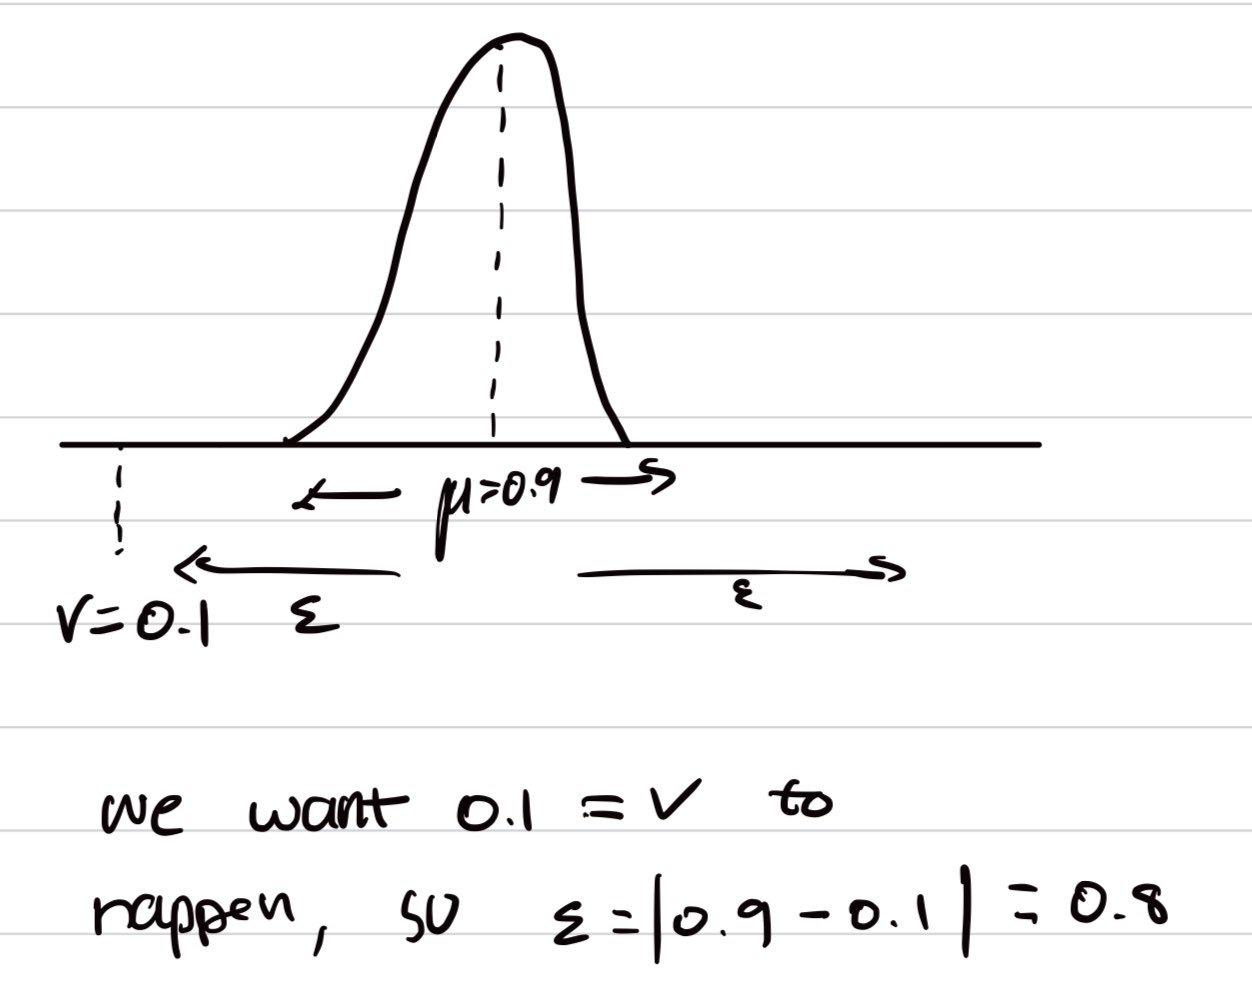
\includegraphics[scale=0.2]{images/1.9.jpg}\\[0.25in]
        Using $P[ |\nu - \mu| \geq \epsilon] \leq 2e^{-2\epsilon^2N}$, we can find the following bounds:\\
        Using $\epsilon = 0.8$ and $N = 10$, we can derive $2e^{-2\epsilon^2N} = 2e^{2(0.8)^2 \times 10}$, which equals $5.52 \times 10^{-6}$.\\
        Since this is a bound, it is reasonable for it to be greater than our answer in exercise 1.8

        \item Exercise 1.10 in LFD
        \begin{enumerate}[label=(\alph*)]
            \item $\mu = 0.5$
            \item \textbf{FINISH HERE}
            \item \textbf{FINISH HERE}
            \item $c_1$ and $c_{rand}$ obey the Hoeffding bound, $c_{min}$ does not because $c1$ and $c_{rand}$ were selected without looking at the data, while $c_{min}$ looks at the data before selecting. $c_{min}$ represents the "unlucky" choice
            \item \textbf{FINISH HERE}
        \end{enumerate}

        \item Exercise 1.11 in LFD
        \begin{enumerate}[label=(\alph*)]
            \item \textbf{FINISH HERE}
            \item \textbf{FINISH HERE}
            \item \textbf{FINISH HERE}
            \item \textbf{FINISH HERE}
        \end{enumerate}

        \item Exercise 1.12 in LFD
        \begin{enumerate}[label=(\alph*)]
            \item \textbf{FINISH HERE}
        \end{enumerate}
    \end{enumerate}
\end{document}